Hier wird die Kaskadierungsvariante des Direct Cascade vorgestellt. 
Das Netzwerk ist hier vorher vollständig und besteht aus einem einzigen Hidden Layer und einem Output Layer. 
Es wird dasselbe Netz mehrfach trainiert und während-dessen wird das Wissen zwischen diesen Netzen weitergegeben. 

\begin{figure}[htpb]
    \centering
    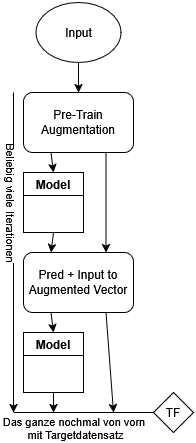
\includegraphics[height=10cm]{../../Graphiken/direct_cascade.png}
    \caption{\label{fig:directcascade} 
    \small{Hier zu sehen ist das Direct Cascade Verfahren. Dieses benutzt mehrere Netzwerke (hier Models), die alle nur sehr wenige 
    Hidden Layer haben, meistens nur eines. Danach wird dieses einmal ohne Training angewandt und dessen Ergebnis mit dem Input verknüpft. 
    Diese Verknüpfung ist der neue Input des nächsten Netzwerkes. Dadurch lernt das Verfahren zwischen den Netzwerken. }}
\end{figure}

Es beginnt, wie in Figure 2.2 gezeigt mit dem präpariertem Sourcedatensatz, der in die Instanz des Netzes hineingegeben wird. 
Damit wird diese Instanz trainiert und sobald dies beendet ist, wird einmal das fixe Netzwerk angewendet. Das Ergebnis davon ist 
die Prediction. Diese wird mit dem Input desselben Netzes verbunden und es entsteht der Augmented Vector. Darauf, wie dieser Augmented 
Vector genau entsteht, wird später nochmal eingegangen, da es bei jedem Direct Cascade Netzwerk ein wenig anders ist. Der Augmented 
Vector wird in die nächste Instanz von dem Netzwerk als input hineingegeben. Die Netzinstanzen, das Training, die Prediction und 
Berechnung der Augmented Vectors wird beliebig häufig wiederholt. Dabei lernt das Netzwerk über den Augmented Vector das Wissen 
der vorherigen Netzwerke mit, da dieses als Prediction dort mit vorkommt. 

TF kann nun jederzeit im Trainingsschritt gemacht werden, indem dort der Targetdatensatz statt der Sourcedatensatz als Input genommen 
wird. Dabei können beliebig viele Netzwerke vor und nach TF genutzt werden. Der einzige Unterschied ist der, dass der Augmented Vector 
für jedes Netzwerk ein wenig größer wird, da dieser sowohl das Wissen von jedem bisherigen Netzwerk als auch die Ursprungsdaten enthält. 

Dabei muss hier in der Implementation bereits von Anfang an sowohl der Sourcedatensatz als auch der Targetdatensatz in das feste Netz 
hineingegeben werden, um die Prediction auf dem Targetdatensatz von der Trainingsphase des Sourcedatensatzes im Augmented Vector zu 
integrieren, damit die Netzwerke, die auf dem Sourcedatensatz gelernt haben, während dem Training auf dem Targetdatensatz Berücksichtigung finden. 
